% OEM briefing deck. Build: latexmk -pdf -outdir=build oem-slides.tex
% Figures are the study's own auto-generated PDFs (norm N4): no slide carries a
% number the pipeline did not produce.
\documentclass[aspectratio=169,11pt]{beamer}
\usetheme{metropolis}
\metroset{sectionpage=progressbar, numbering=fraction, progressbar=frametitle, block=fill}
\usepackage[utf8]{inputenc}
\usepackage[T1]{fontenc}
\usepackage{lmodern}
\usepackage[english]{babel}
\usepackage{amsmath,amssymb}
\usepackage{booktabs}
\usepackage{graphicx}
\graphicspath{{../report/figures/}}
\definecolor{inkc}{HTML}{212529}
\definecolor{bluec}{HTML}{4263EB}
\definecolor{redc}{HTML}{A61E4D}
\definecolor{grayc}{HTML}{868E96}
\setbeamercolor{frametitle}{bg=inkc}
\setbeamercolor{progress bar}{fg=bluec}
\setbeamercolor{alerted text}{fg=redc}
\newcommand{\lead}[1]{{\footnotesize\itshape\color{grayc}#1}\par\smallskip}

\title{Which AI claims in engine performance survive testing?}
\subtitle{A measurement rig --- and what it found, including about our own numbers}
\date{}
\author{}

\begin{document}
\maketitle

\begin{frame}{Start from the skeptical position, because the data supports it}
  \lead{This is not a pitch. It is an audit, and most of what was audited failed.}
  \begin{columns}[T]
    \begin{column}{0.5\textwidth}
      \textbf{What we set out to test}
      \begin{itemize}
        \item Does AI beat a \emph{tuned} classical gas-path stack?
        \item Same data, same metrics, same tuning budget
        \item Hypotheses frozen \alert{before} the runs
        \item Ground truth known, so a diagnosis is scored against the answer
      \end{itemize}
    \end{column}
    \begin{column}{0.5\textwidth}
      \textbf{What came back}
      \begin{itemize}
        \item A published result's headline claim: \alert{noise}
        \item Two of \emph{our own} headlines: \alert{cut by 3--4$\times$}
        \item The task AI is most sold for: \alert{dead heat}
        \item ``Physics-informed AI'': \alert{refuted twice}
      \end{itemize}
      \medskip
      {\small The part that survived points at \textbf{instrumentation}, not software.}
    \end{column}
  \end{columns}
\end{frame}

\begin{frame}{The rig, in one slide}
  \lead{Everything from public certification data --- TCDS and ICAO EEDB. No proprietary inputs.}
  \begin{itemize}
    \item Thermodynamic model of a CFM56-7B26, calibrated to certification test-bed data
    \item 100-engine synthetic fleet run to failure, with \textbf{true} component condition recorded per flight
    \item Two tuned practitioners: classical Kalman gas-path analysis, and a matched AI suite
    \item Airline-format data: two snapshots per flight, cockpit sensors only
  \end{itemize}
  \vspace{2mm}
  \begin{alertblock}{Why ground truth is the whole point}
    On real data you can only compare one estimate against another. Here we can ask
    the question that matters: \emph{was the diagnosis right?}
  \end{alertblock}
\end{frame}

\section{What failed}

\begin{frame}{A peer-reviewed deep-learning result, replicated exactly}
  \lead{Springer 2026: a bidirectional LSTM, ``best of fifteen architectures'' for remaining life.}
  \begin{columns}[T]
    \begin{column}{0.52\textwidth}
      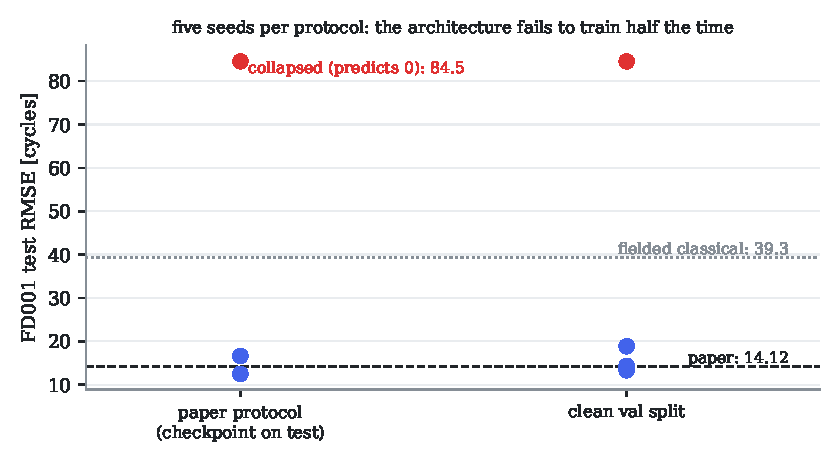
\includegraphics[width=\linewidth]{f14_bilstm}
    \end{column}
    \begin{column}{0.46\textwidth}
      \textbf{It replicates.} 14.56 cycles against a reported 14.12. Not a straw man.
      \medskip

      \textbf{But:} the 15-way ranking rests on gaps of \alert{0.12--0.60} cycles.
      Seed-to-seed spread alone is \alert{2.94}. The ranking is noise --- one run per model.
      \medskip

      \textbf{And:} the published architecture \alert{fails to train on 5 of 10 runs},
      predicting zero. Cause is in the paper's own tables.
    \end{column}
  \end{columns}
\end{frame}

\begin{frame}{The evaluation question to ask anyone, including us}
  \begin{block}{Before you look at the headline}
    \Large\centering ``What is the seed spread?''
  \end{block}
  \vspace{3mm}
  \begin{itemize}
    \item A ranking inside the run-to-run noise is not a result
    \item A model that silently fails half the time is not a product
    \item One run per architecture cannot support a ranking of fifteen
  \end{itemize}
  \vspace{2mm}
  \lead{This alone is worth having when the next vendor deck arrives.}
\end{frame}

\begin{frame}{We applied it to our own claims, and both shrank}
  \begin{columns}[T]
    \begin{column}{0.5\textwidth}
      \textbf{``6$\times$ tighter uncertainty''}
      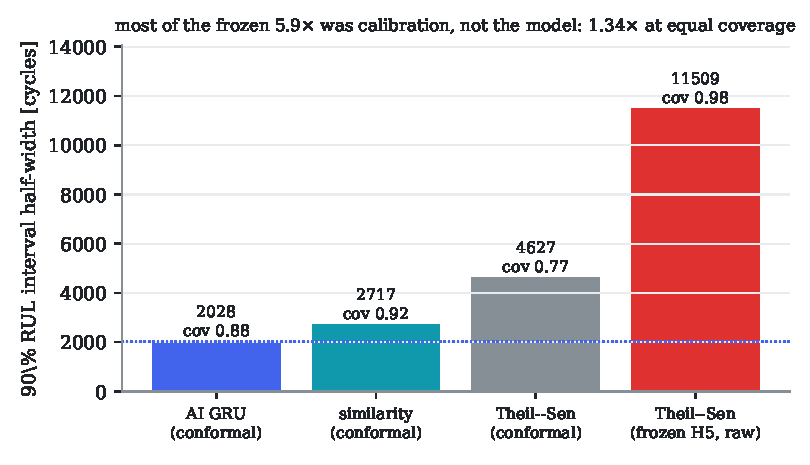
\includegraphics[width=\linewidth]{uq_reattribution}
      {\footnotesize Our interval was statistically calibrated; theirs was not.
      Calibrate both --- free to the classical side --- and it is
      \alert{1.34$\times$}.}
    \end{column}
    \begin{column}{0.5\textwidth}
      \textbf{``2.3--4.4$\times$ better remaining life''}
      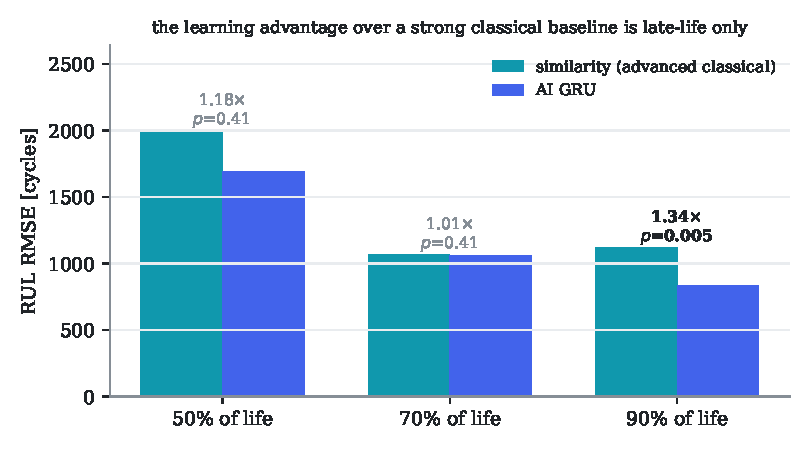
\includegraphics[width=\linewidth]{lrul_sweep}
      {\footnotesize True only against the linear extrapolation fielded today.
      Against a competent classical method: \alert{1.34$\times$ late in life, a
      tie at 70\,\%}.}
    \end{column}
  \end{columns}
\end{frame}

\begin{frame}{Where AI lost outright --- and why no algorithm fixes it}
  \lead{Isolating confusable gas-path faults: 31\,\% vs 31\,\%. Identical.}
  \begin{columns}[T]
    \begin{column}{0.48\textwidth}
      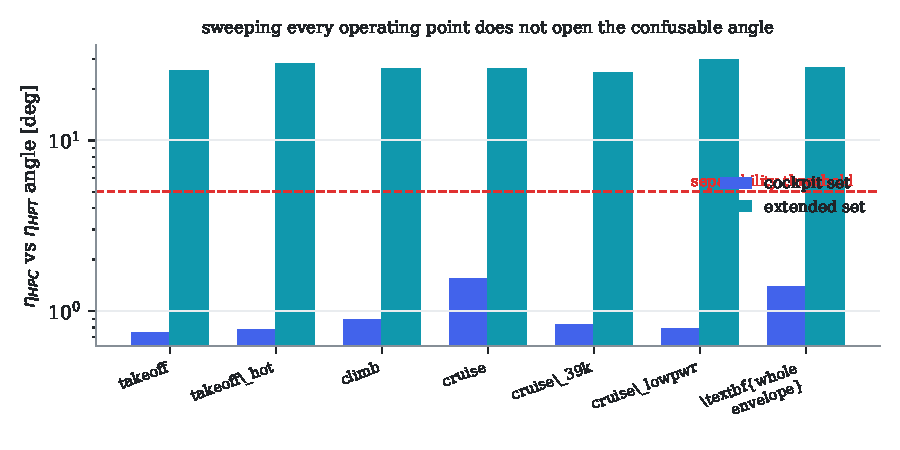
\includegraphics[width=\linewidth]{gate_t}
    \end{column}
    \begin{column}{0.5\textwidth}
      Three cockpit measurements, ten health parameters, two fault signatures
      \alert{$1.3^{\circ}$} apart. Confirmed four independent ways:
      \begin{itemize}\small
        \item halve every sensor noise $\rightarrow$ still 0.31--0.38
        \item add a ``virtual sensor'' $\rightarrow$ \alert{exactly zero}
        \item sweep the whole operating envelope $\rightarrow$ $1.38^{\circ}$
        \item every learned method $\rightarrow$ no movement
      \end{itemize}
      \medskip
      \begin{alertblock}{}
        \centering No algorithm removes a rank deficiency.
      \end{alertblock}
    \end{column}
  \end{columns}
\end{frame}

\begin{frame}{And most prognostic error is not a method gap}
  \begin{block}{87\,\% of mid-life remaining-life uncertainty is irreducible}
    Two engines in \emph{identical measured condition} genuinely fail hundreds of
    cycles apart. We can measure this because we know the true condition.
  \end{block}
  \vspace{3mm}
  \begin{itemize}
    \item Late in life a $4\times$ reducible gap opens --- \textbf{that} is where a
          better prognostic pays
    \item Early in life, a better algorithm is chasing the future, not a deficiency
  \end{itemize}
  \vspace{2mm}
  \lead{A budget question answered with a number instead of an opinion.}
\end{frame}

\section{What survived}

\begin{frame}{An instrumentation design tool --- and it is not AI}
  \lead{Classical estimation theory through the engine deck, checked against true condition.}
  Accumulate Fisher information over an engine's actual flown conditions
  $\Rightarrow$ a per-direction bound on what \emph{any} diagnosis can know.
  \vspace{2mm}
  \begin{center}\small
  \begin{tabular}{@{}lr@{}}
    \toprule
    Instrumentation decision & Measured effect \\
    \midrule
    Add station probes (P25/T25/PS3/T3) & HPC efficiency \alert{45$\times$} better recovered \\
    Same probes, confusable isolation & \alert{0.15 $\rightarrow$ 0.92} \\
    Halve noise on existing cockpit probes & no effect \\
    ``Virtual sensor'' or better algorithm & no effect \\
    \bottomrule
  \end{tabular}
  \end{center}
  \vspace{2mm}
  \lead{It prices the hardware decision before the hardware is committed.}
  \vspace{1mm}
  {\scriptsize\color{grayc} Honest caveat: the ranking claim behind this tool
  ($\rho = 0.70$ against true error) is real signal but does not clear its own
  physics-free null ($0.24$ median, $p = 0.085$) --- the \emph{acquisition} numbers
  above are separate measurements and are unaffected.}
\end{frame}

\begin{frame}{Why this one is ours to act on}
  \begin{alertblock}{Product-strategy consequence}
    Any EHM service built on \textbf{cockpit-only data} sits under a hard
    informational ceiling that no software roadmap removes.
  \end{alertblock}
  \vspace{3mm}
  \begin{itemize}
    \item The way through is \textbf{instrumentation} --- which an OEM controls and a customer does not
    \item The analysis runs on \textbf{our own decks}, where it is stronger than on the public model used here
    \item It needs \textbf{no AI and no new data collection}
  \end{itemize}
\end{frame}

\begin{frame}{The one AI result that held up}
  \lead{And it is narrower and more useful than the usual claim.}
  \begin{columns}[T]
    \begin{column}{0.46\textwidth}
      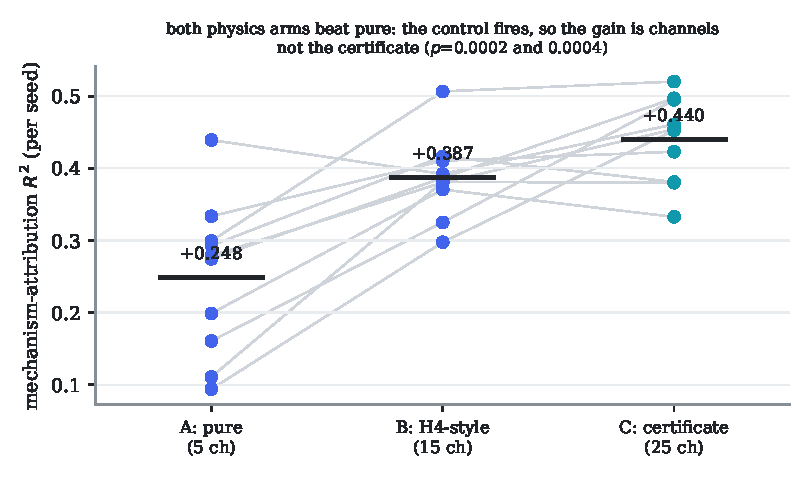
\includegraphics[width=\linewidth]{hybrid_arms}
    \end{column}
    \begin{column}{0.52\textwidth}
      Injecting physics into a learner:
      \begin{itemize}
        \item \alert{hurts} remaining-life prediction (refuted twice)
        \item \textbf{helps} module attribution, by a large significant margin
      \end{itemize}
      \medskip
      Run with a \textbf{control arm}, so the gain cannot be attributed to simply
      adding more inputs.
      \medskip

      {\small Remaining life is already carried by the EGT-margin signal the model sees.
      \emph{Which module} is exactly what a physical state estimate encodes.}
      \medskip

      \begin{block}{}\centering The task decides.\end{block}
    \end{column}
  \end{columns}
\end{frame}

\begin{frame}{What this is, and what it is not}
  \begin{columns}[T]
    \begin{column}{0.48\textwidth}
      \textbf{\alert{Not}}
      \begin{itemize}
        \item A product or a validated operational tool
        \item Evidence about absolute numbers --- the fleet is synthetic and the
              model is calibrated to public data, not our test cell
        \item A certified conclusion. These are statistical predictions
      \end{itemize}
    \end{column}
    \begin{column}{0.48\textwidth}
      \textbf{Is}
      \begin{itemize}
        \item A reusable method for deciding which performance-AI claims to fund
              and which to reject
        \item Hypotheses frozen before runs; equal tuning budgets both sides
        \item Negatives reported with the same weight as positives
        \item Every figure regenerated from data, never transcribed
      \end{itemize}
    \end{column}
  \end{columns}
\end{frame}

\begin{frame}[standout]
  Proposed next step

  \vspace{4mm}
  {\large Re-run the instrumentation analysis on our own engine decks
  and our own candidate sensor suites.}

  \vspace{4mm}
  {\normalsize No AI. No new data collection. Answers a question we already pay
  to answer by other means.}
\end{frame}

\appendix

\begin{frame}{Backup --- the discipline that makes the answers usable}
  \begin{itemize}
    \item \textbf{Pre-registration}: every hypothesis and threshold frozen in a
          tagged document before the run; refutations recorded, never renegotiated
    \item \textbf{Symmetric budgets}: both method families get the same number of
          tuning trials. Untuned comparisons inverted our own early scoreboard
    \item \textbf{Gates allowed to fail}: the dataset difficulty gate failed twice
          and the data was fixed, not the threshold
    \item \textbf{Built-in fraud checks}: give a method a case where physics says
          the information cannot exist, and confirm it finds nothing
    \item \textbf{Auto-generated figures}: no number reaches a slide without
          coming from the pipeline
  \end{itemize}
\end{frame}

\begin{frame}{Backup --- the wall is a snapshot property}
  \lead{Three of five degradation mechanisms are attributable from the trajectory shape.}
  \begin{columns}[T]
    \begin{column}{0.55\textwidth}
      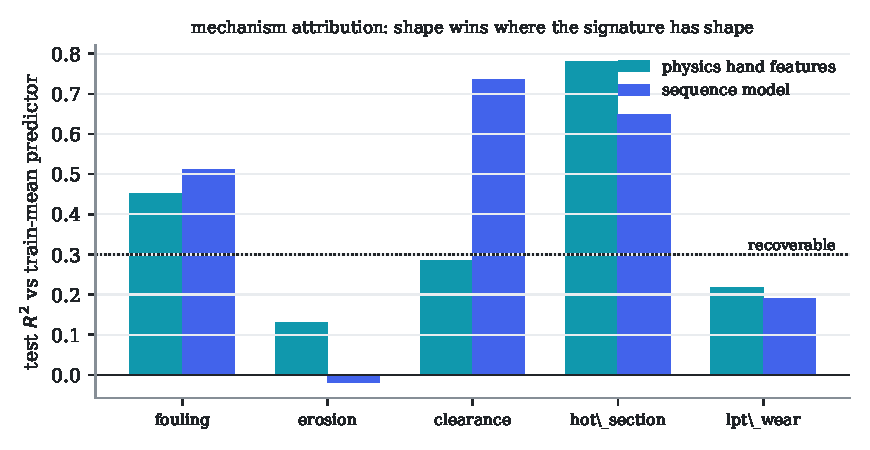
\includegraphics[width=\linewidth]{f13_mechanism}
    \end{column}
    \begin{column}{0.43\textwidth}
      Including the hot-section mechanism that drives the confusable pair
      ($R^2 = 0.78$).
      \medskip

      \begin{block}{The rule we measured}
        Trajectory shape separates \textbf{what has shape}.
      \end{block}
      \medskip
      {\small A wash sawtooth and a break-in knee are readable. A featureless
      linear ramp is not, however long you watch --- which is also why a drifting
      sensor cannot be told from a real fault.}
    \end{column}
  \end{columns}
\end{frame}

\end{document}
